\section{Detail of Directmap Join}
    This appendix describes the implementation of \textit{directmap join}.\par
    In the build phase, we copy inner relation into a two-dimension-al array called \textit{map}, which can be treated as a special hash table with the data of inner relation. The hash function of \textit{map} is $hash(x)=x$. Note that this simple hash function only works when the join attribute value is a non-negative integer, which is satisfied in JOB but not in all benchmarks. And each row of \textit{map} is used to store a data tuple, and by given hash function, the data tuple is stored at the row whose row number equals the value of the data tuple's join attribute.\par
    Except for data slot, each row of the \textit{map} calso contains a header. Header consists of three components: \textit{valid}, \textit{previous}, and \textit{next}. \textit{va-lid} represents if the data slot has been occupied by an inner tuple. However, it is common that several tuples have the same value on the join attribute, which causes a conflict. We use open addressing \cite{book2} to solve this problem. And we use \textit{previous} and \textit{next} to maintain a list where all members have the same join attribute value, in order to avoid unnecessary search in the \textit{map}. When meet a conflict, we store the new tuple in an empty row and add its position to the tail of corresponding list. Moreover, if there is no more empty row for the new-coming tuple, we simply double the size of \textit{map}.\par
    We fetch inner tuple from scan operator one by one to create \textit{map}. When an inner table tuple $t_1$ comes, we first calculate the row number that it will store in according to its join attribute value. Then we check \textit{valid} to ensure the target row is empty and there would be three cases:\par
    \textbf{Case 1}: If \textit{valid} is 0, we store $t_1$ in the target row and set \textit{previous} and \textit{next} to $N/A$.\par
    \textbf{Case 2} (Figure \ref{F18}): If \textit{valid} is 1, which means the row is occupied by a tuple $t_2$. Meanwhile, $t_2$ is a ``host tuple" whose join attribute value equals to its row number. Then, we place tuple $t_1$ to an empty row and call tuple $t_1$ as ``guest tuple" whose join attribute value does not equal to its row number. And we add its position to the tail of list where the join attribute value of tuples equals to $t_1$.
    \begin{figure}[htb]
        \centering
        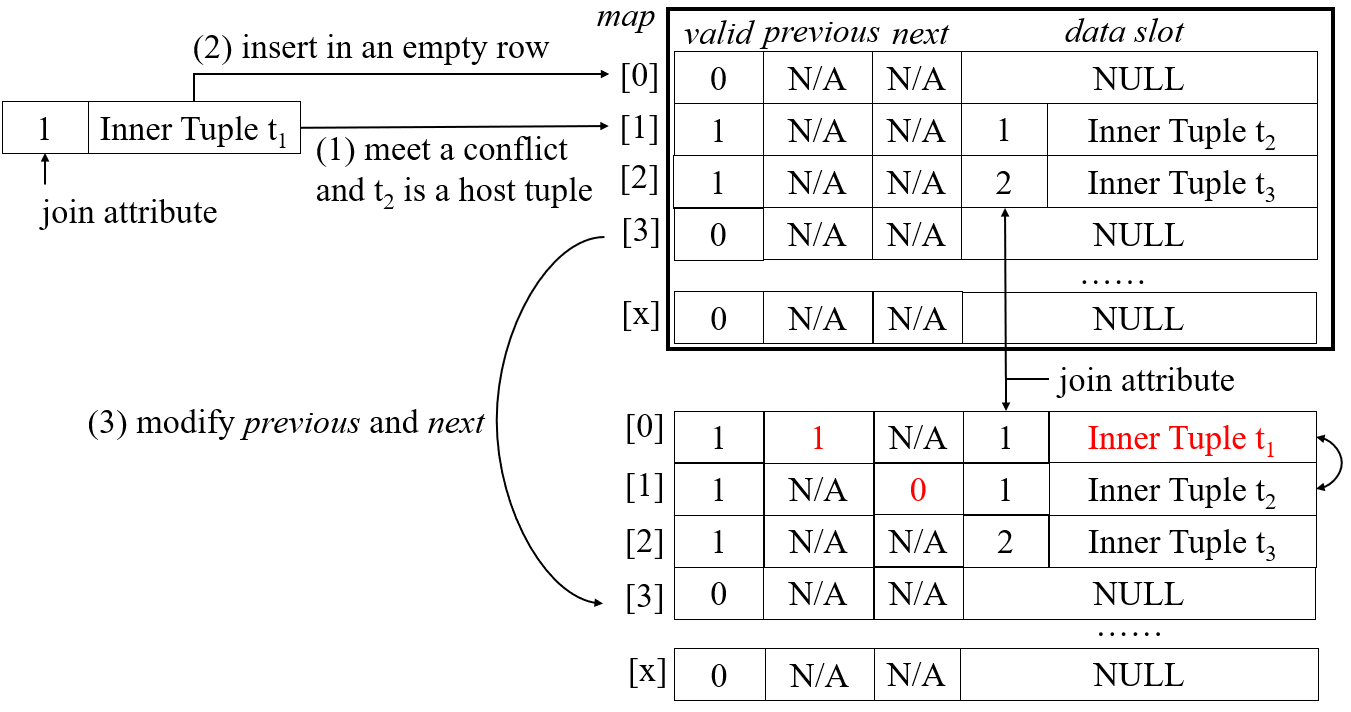
\includegraphics[width=\linewidth]{./pic/Figure18.png}
        \caption{The illustration of condition 2}
        \label{F18}
        \Description{}
    \end{figure}\par
    \textbf{Case 3} (Figure \ref{F19}): If \textit{valid} is 1 and $t_2$ is a ``guest tuple", whose join attribute value does not equal to its row number. We first move $t_2$ to a new empty row, then fit $t_1$ in this row as ``host tuple" and set the \textit{previous} and \textit{next} to $N/A$. Then, we refresh the position of $t_2$ in the list where all members have the same join attribute value with $t_2$.
    \begin{figure}[htb]
        \centering
        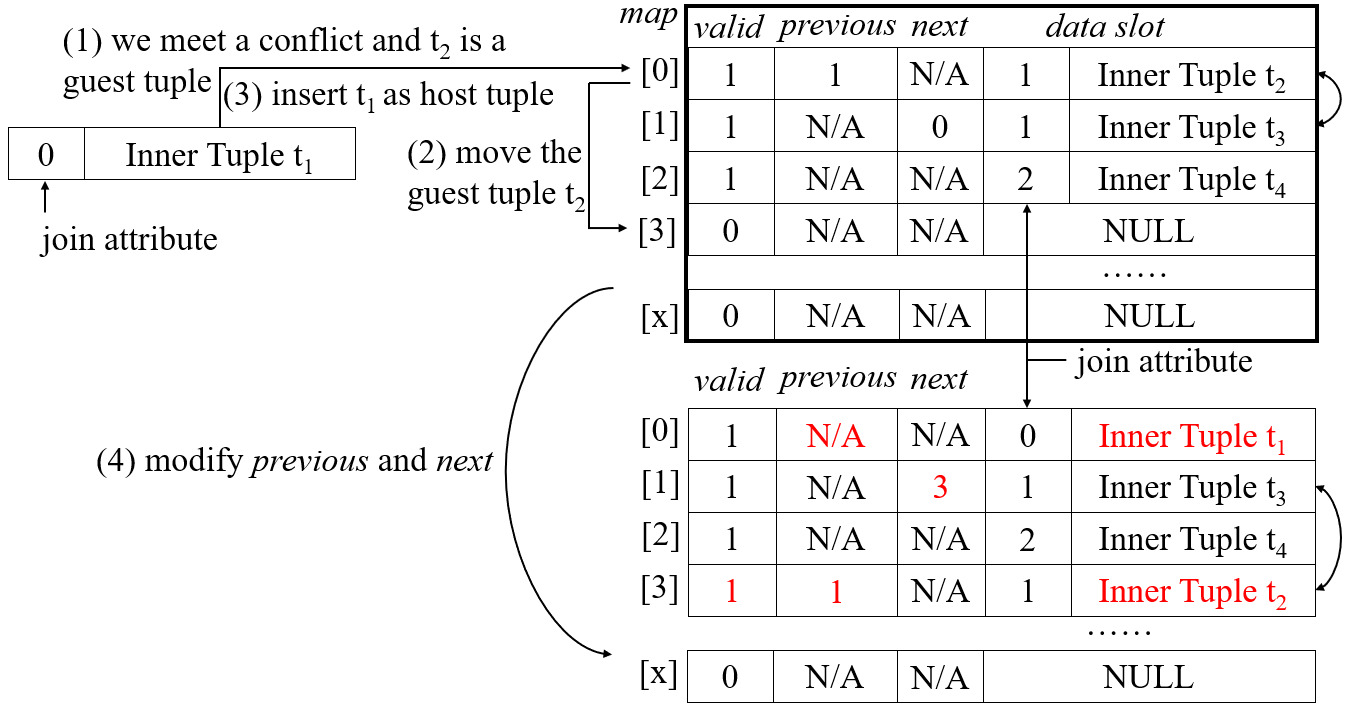
\includegraphics[width=\linewidth]{./pic/Figure19.png}
        \caption{The illustration of condition 3}
        \label{F19}
        \Description{}
    \end{figure}\par
    After introducing how to build \textit{map}, we describe how to return a join result in probe phase. As shown in Figure \ref{F20}, we first fetch an outer tuple, and then we get the join attribute value of outer tuple as row number to fetch the corresponding row in \textit{map}. After we fetch the corresponding row from \textit{map}, we check its \textit{valid word}. If empty, we fetch the next outer tuple and repeat above steps. Otherwise, we check \textit{next} to determine whether there is a list. If $N/A$, which means there is only one tuple has given join attribute value, we return the join result and fetch next outer tuple. If not $N/A$, we not only return the join result, but also fetch the successors that have the same join attribute value by traversing the list.
    \begin{figure}[htb]
        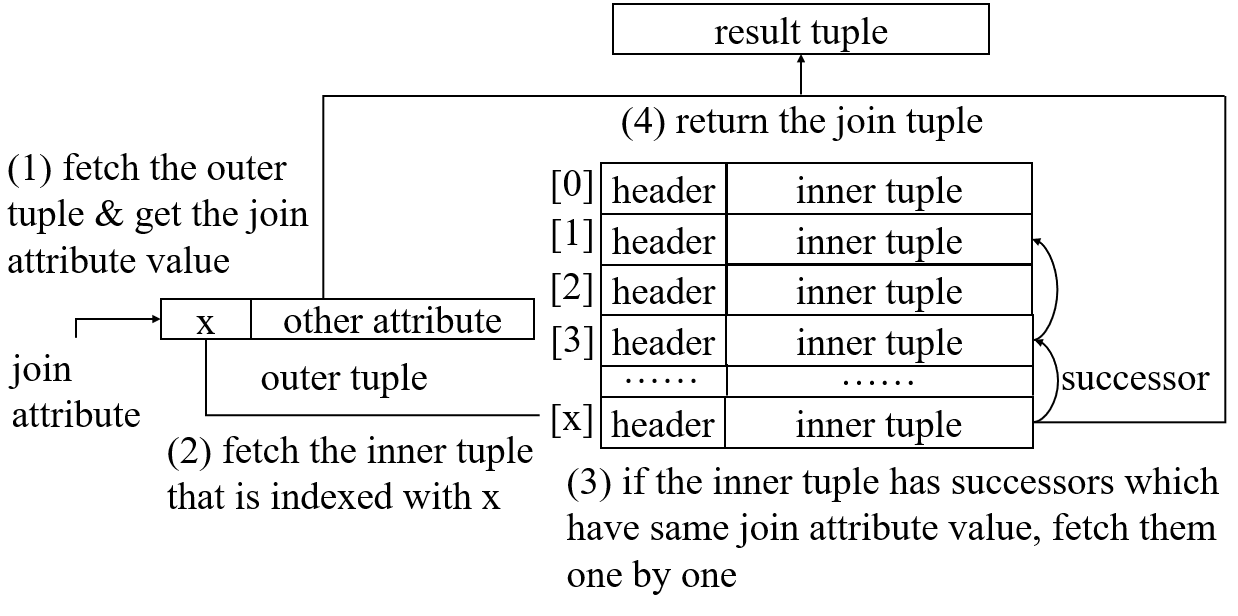
\includegraphics[width=\linewidth]{./pic/Figure20.png}
        \caption{How \textit{directmap join} works}
        \label{F20}
        \Description{}
    \end{figure}\par
    Another problem is how to combine \textit{directmap join} with PostgreSQL optimizer. By our design, whether the optimizer chooses the \textit{directmap join} operator depends on a heuristic judgment and its cost model.\par
    A heuristic judgment is used to control the memory usage, as the size of \textit{map} is no less than the maximum of join attribute, which means \textit{directmap join} sacrifices memory to earn speed. First, we ensure that the inner relation must be a base relation or a subquery result to avoid too much confliction. Then, we check the ratio $t=f_r/n_r$, where $f_r$ is the estimated number of tuples after applying the predicate on inner relation, and $n_r$ is the size of inner relation. As \textit{map} size is no less than the maximum of appeared join attribute values, we use $n_r$ to approximate the \textit{map} size. And $f_r$ equals the number of rows that we actually use in \textit{map}. Hence, the ratio can roughly estimate the ratio of how much memory that we actually use for storage and allocate for \textit{directmap join}, which reflects the memory utilization rate of \textit{directmap join}. If the ratio is less than a threshold, we think it's memory-wasteful to create a \textit{map}, so we abandon the consideration of using \textit{directmap join}.\par
    Second, we set the cost model of \textit{directmap join} by imitating the cost model of \textit{hash join}. As \textit{directmap join} reduced twice memory access to once, we half the fetch cost by CPU. To show our change in fetch cost, we divide the cost of \textit{hash join} by two as the cost of \textit{directmap join}.